\section{Results}
\label{sec:results}

All values below are means $\pm$ standard deviations across random seeds unless stated otherwise.

% ------------------------------------------------------------------
\subsection{Overall Prediction Accuracy}
\label{sec:results_prediction}

Table~\ref{tab:grand_summary} gives the big picture.
The two Bayesian methods lead on prediction error (MSE around 72), roughly 35\% lower than Lasso and Elastic Net (around 108), and far ahead of OLS (267).
Ridge lands in the middle at 119.

\begin{table}[ht]
\centering
\caption{Aggregate performance across all synthetic experiments.}
\label{tab:grand_summary}
\begin{tabular}{lccc}
\toprule
Model & Test MSE & Coef. $L_2$ Error & Support $F_1$ \\
\midrule
OLS & 267.159 $\pm$ 323.478 & 16.559 $\pm$ 14.988 & 0.296 $\pm$ 0.026 \\
Ridge & 118.597 $\pm$ 124.690 & 6.405 $\pm$ 2.902 & 0.297 $\pm$ 0.027 \\
Lasso & 108.101 $\pm$ 121.213 & 5.199 $\pm$ 3.311 & 0.470 $\pm$ 0.132 \\
Elastic Net & 108.751 $\pm$ 122.784 & 5.209 $\pm$ 3.248 & 0.459 $\pm$ 0.126 \\
Horseshoe & 71.917 $\pm$ 76.047 & 4.210 $\pm$ 2.630 & 0.288 $\pm$ 0.037 \\
Spike-and-Slab & 72.992 $\pm$ 78.317 & 4.588 $\pm$ 3.041 & 0.469 $\pm$ 0.156 \\
\bottomrule
\end{tabular}
\end{table}

Figure~\ref{fig:mse_vs_snr} breaks this down by dataset and SNR.
At high SNR ($\geq 5$), most regularized methods converge to similar MSE levels.
The differences emerge at low SNR, where the adaptive shrinkage of Bayesian priors---especially Horseshoe---pays off.
OLS is consistently the worst, as expected for an unregularized estimator.

\begin{figure}[ht]
\centering
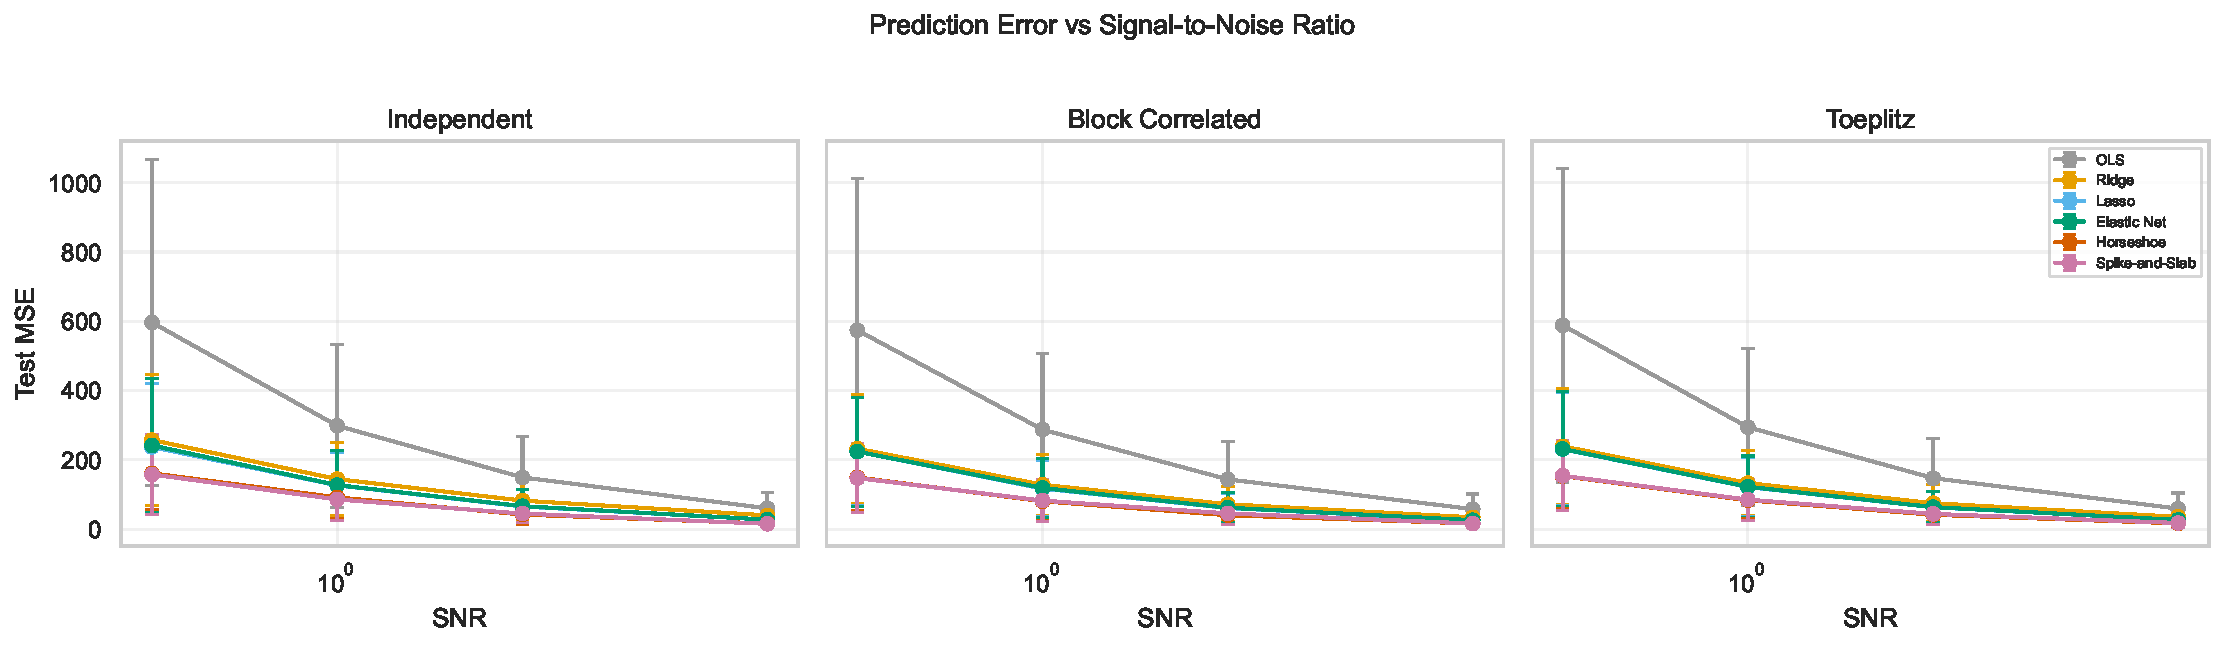
\includegraphics[width=\textwidth]{figures/lineplot_mse_vs_snr_by_dataset.pdf}
\caption{Test MSE vs.\ SNR for each covariance design. Error bars: $\pm 1$ std across seeds.}
\label{fig:mse_vs_snr}
\end{figure}

% ------------------------------------------------------------------
\subsection{Robustness to Feature Correlation}
\label{sec:results_correlation}

Figure~\ref{fig:mse_vs_corr} is perhaps the most practically relevant plot in this paper.
It shows what happens to each method as you crank up the feature correlation.

\begin{figure}[ht]
\centering
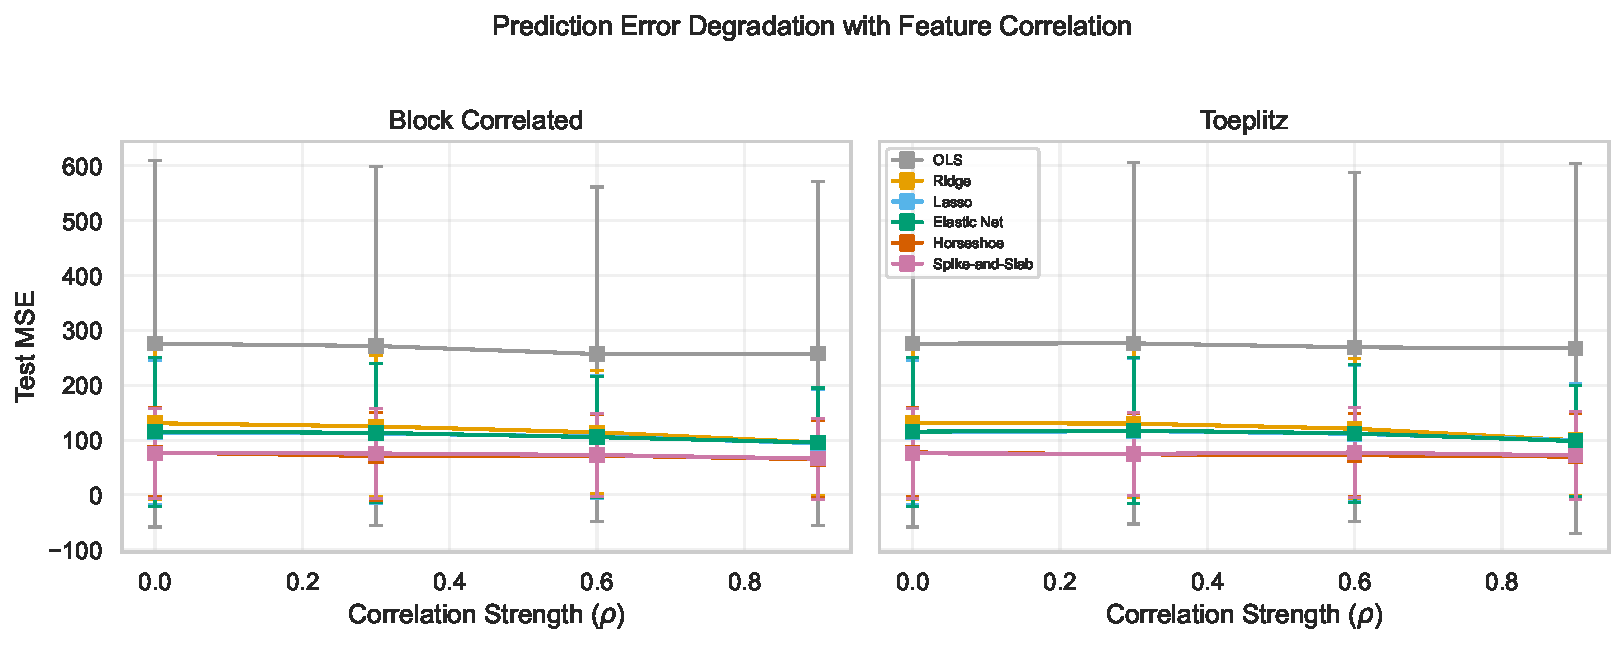
\includegraphics[width=\textwidth]{figures/lineplot_mse_vs_correlation.pdf}
\caption{MSE degradation with increasing $\rho$. Left: Block Correlated. Right: Toeplitz.}
\label{fig:mse_vs_corr}
\end{figure}

OLS falls apart first---its MSE climbs steeply beyond $\rho = 0.3$.
Ridge and Elastic Net hold up reasonably well thanks to their $\ell_2$ component.
Lasso degrades noticeably at $\rho \geq 0.6$: correlated features confuse its variable selection, and the resulting coefficient instability hurts prediction.
The Horseshoe prior is the most robust here, with its local-global shrinkage adapting to the correlation structure.

The Toeplitz design tells a similar story but with a smoother degradation curve, since correlations decay with distance between features rather than cutting off at block boundaries.

\begin{figure}[ht]
\centering
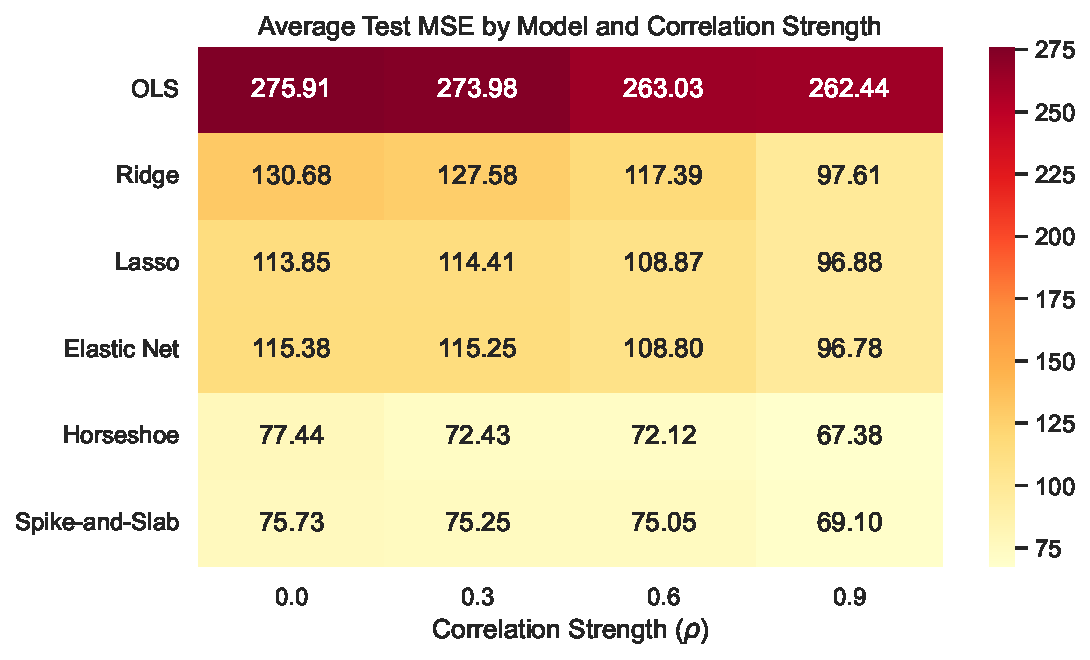
\includegraphics[width=0.75\textwidth]{figures/heatmap_mse_vs_correlation.pdf}
\caption{MSE heatmap: model $\times$ correlation strength.}
\label{fig:mse_heatmap}
\end{figure}

% ------------------------------------------------------------------
\subsection{Variable Selection}
\label{sec:results_selection}

Figure~\ref{fig:f1_vs_snr} shows $F_1$ scores for support recovery.

\begin{figure}[ht]
\centering
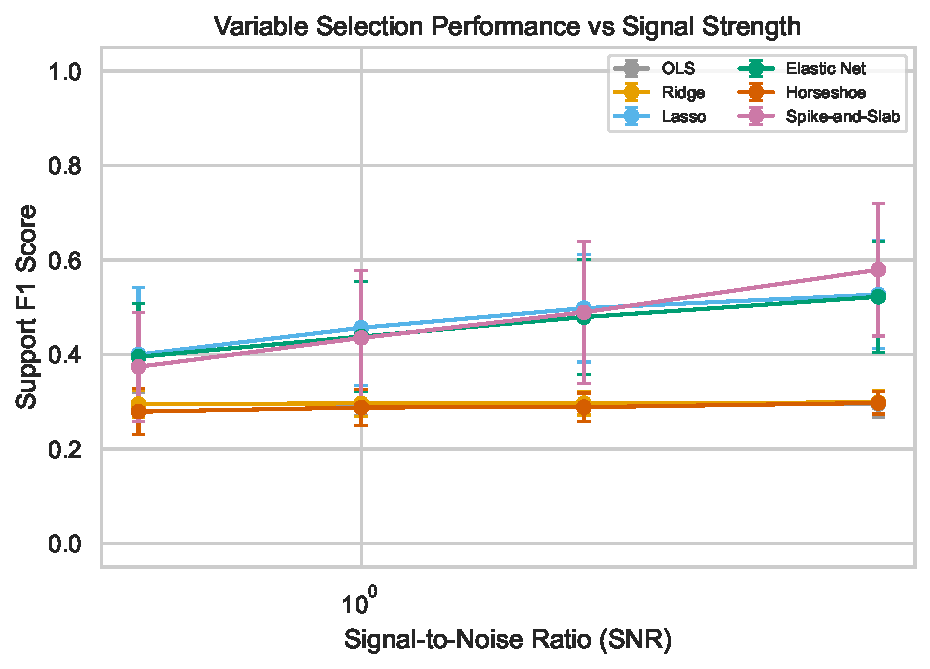
\includegraphics[width=0.7\textwidth]{figures/lineplot_f1_vs_snr.pdf}
\caption{Support recovery $F_1$ vs.\ SNR.}
\label{fig:f1_vs_snr}
\end{figure}

Two methods stand out: Lasso and Spike-and-Slab, both reaching $F_1 \approx 0.47$ on average.
Elastic Net is close behind.
OLS and Ridge are stuck around $F_1 = 0.30$ because they assign nonzero weights to almost every feature (high recall, low precision).
The Horseshoe, despite its strong prediction performance, is surprisingly mediocre at hard thresholding---its posterior means are shrunken but rarely exactly zero, so the $|\hat{\beta}_j| > 0.01$ threshold does not serve it well.
A more Bayesian selection rule (e.g., based on credible intervals excluding zero) would likely improve its $F_1$.

\begin{figure}[ht]
\centering
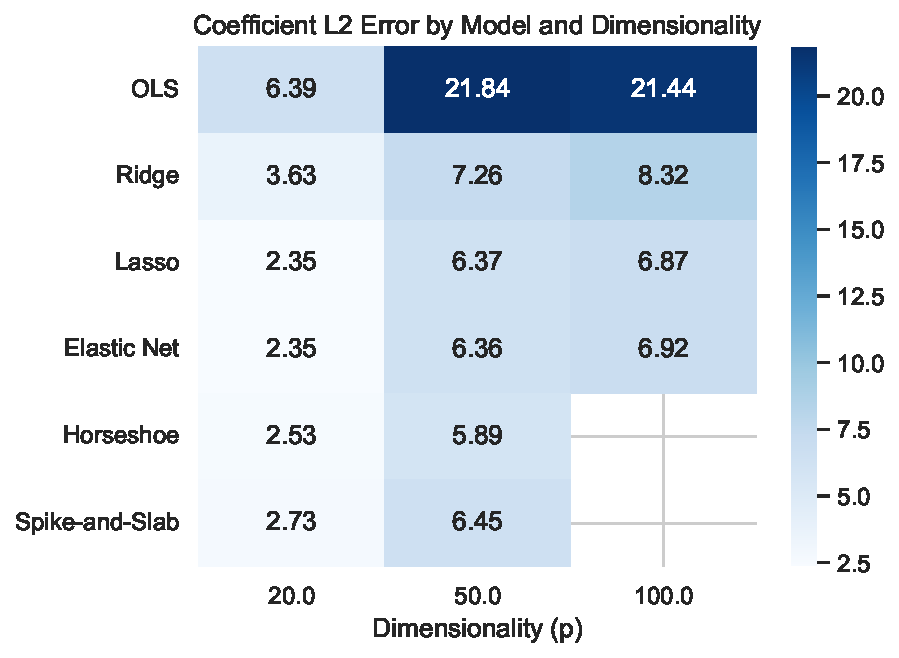
\includegraphics[width=0.65\textwidth]{figures/heatmap_l2_vs_dim.pdf}
\caption{Coefficient $L_2$ error by model and dimensionality.}
\label{fig:l2_heatmap}
\end{figure}

On raw coefficient estimation (Figure~\ref{fig:l2_heatmap}), the story favors Bayesian methods more clearly: Horseshoe achieves the lowest $L_2$ error at every dimensionality, followed by Spike-and-Slab and Lasso.

% ------------------------------------------------------------------
\subsection{Uncertainty Quantification}
\label{sec:results_uq}

This is where the Bayesian methods earn their computational cost---or not.

\IfFileExists{figures/barchart_coverage.pdf}{%
\begin{figure}[ht]
\centering
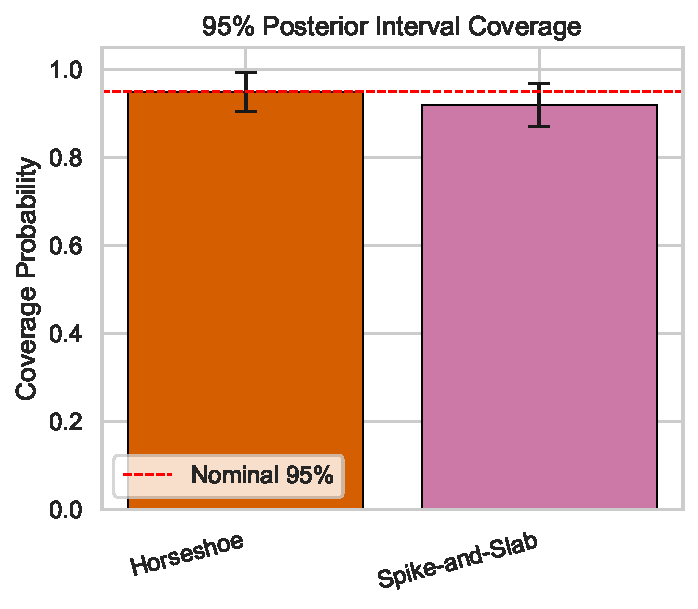
\includegraphics[width=0.45\textwidth]{figures/barchart_coverage.pdf}
\caption{Empirical 95\% HDI coverage. Dashed red line: nominal level.}
\label{fig:coverage}
\end{figure}
}{}

Table~\ref{tab:bayesian_uq} summarizes the calibration results.
The Horseshoe achieves 94.8\% coverage, close to the nominal 95\%---a good result that validates its posterior as trustworthy.
Its intervals are wider on average (2.24), which is the price of honesty: the prior spreads mass conservatively.

Spike-and-Slab, by contrast, under-covers at 91.9\% despite producing narrower intervals (1.06).
We suspect the continuous relaxation is the culprit: the \texttt{NormalMixture} approximation blurs the sharp spike-slab boundary, leading to posteriors that are sometimes too concentrated around the wrong value.
A discrete Gibbs sampler implementation might close this gap, but at further computational cost.

\begin{table}[ht]
\centering
\caption{Bayesian posterior calibration: coverage and interval width.}
\label{tab:bayesian_uq}
\begin{tabular}{lcc}
\toprule
Model & Coverage (95\% HDI) & Avg.\ Interval Width \\
\midrule
Horseshoe & 0.948 $\pm$ 0.045 & 2.237 $\pm$ 1.121 \\
Spike-and-Slab & 0.919 $\pm$ 0.048 & 1.058 $\pm$ 0.865 \\
\bottomrule
\end{tabular}
\end{table}

% ------------------------------------------------------------------
\subsection{Computational Cost}
\label{sec:results_runtime}

\begin{figure}[ht]
\centering
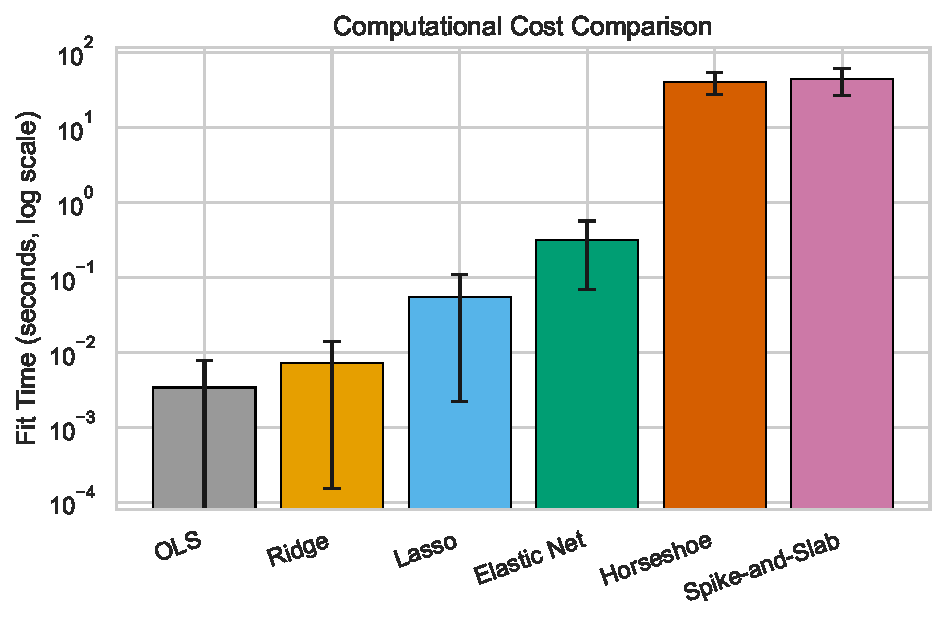
\includegraphics[width=0.6\textwidth]{figures/barchart_runtime.pdf}
\caption{Mean fit time per experiment (log scale).}
\label{fig:runtime}
\end{figure}

The cost gap is stark (Figure~\ref{fig:runtime}).
Classical methods fit in well under one second at all tested dimensions.
Bayesian methods take tens of seconds at $p = 20$ and minutes at $p = 50$, with Spike-and-Slab consistently slower than Horseshoe due to the mixture model's more complex geometry.

% ------------------------------------------------------------------
\subsection{Seed Stability}
\label{sec:results_stability}

\begin{figure}[ht]
\centering
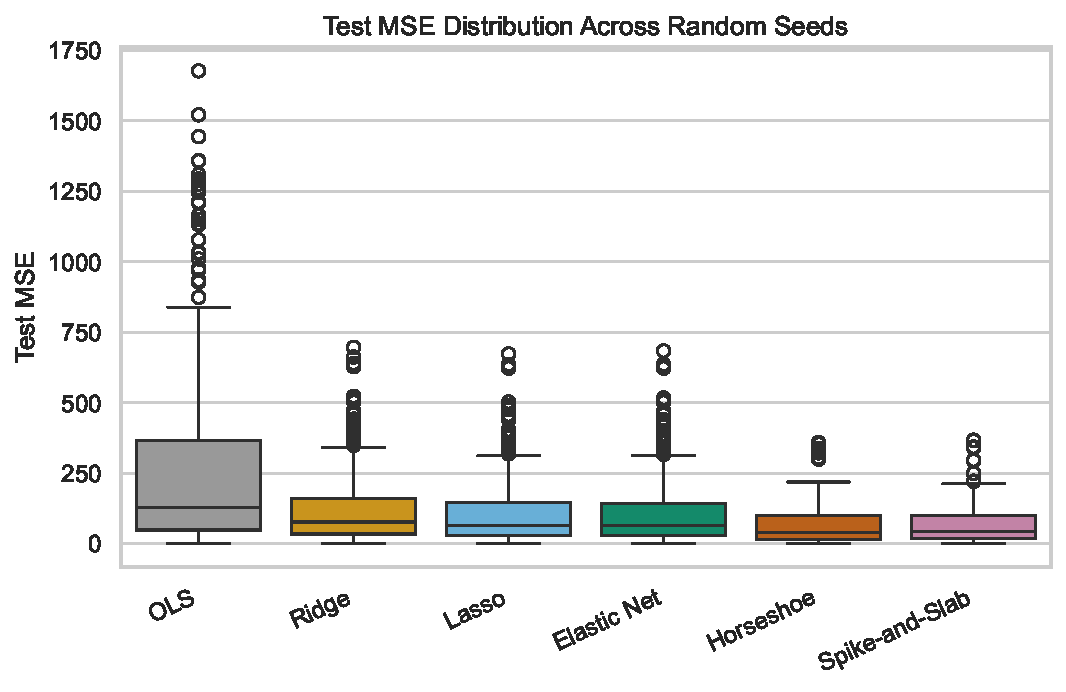
\includegraphics[width=0.7\textwidth]{figures/boxplot_seed_stability.pdf}
\caption{Test MSE spread across random seeds.}
\label{fig:seed_stability}
\end{figure}

Classical methods are nearly deterministic given fixed data (Figure~\ref{fig:seed_stability}).
Bayesian methods show wider boxes due to MCMC randomness, but the spread is modest---not a practical concern with 1{,}000+ posterior draws.

% ------------------------------------------------------------------
\subsection{Real Data: Diabetes}
\label{sec:results_diabetes}

\begin{table}[ht]
\centering
\caption{Diabetes dataset ($n=442$, $p=10$).}
\label{tab:diabetes}
\begin{tabular}{lccc}
\toprule
Model & Test MSE & Test RMSE & Time (s) \\
\midrule
OLS & 0.507 $\pm$ 0.060 & 0.711 $\pm$ 0.041 & 0.00 \\
Ridge & 0.508 $\pm$ 0.057 & 0.712 $\pm$ 0.039 & 0.00 \\
Lasso & 0.504 $\pm$ 0.057 & 0.709 $\pm$ 0.039 & 0.02 \\
Elastic Net & 0.504 $\pm$ 0.057 & 0.709 $\pm$ 0.039 & 0.15 \\
Horseshoe & 0.472 $\pm$ 0.011 & 0.687 $\pm$ 0.008 & 11.71 \\
Spike-and-Slab & 0.473 $\pm$ 0.008 & 0.688 $\pm$ 0.006 & 12.51 \\
\bottomrule
\end{tabular}
\end{table}

With only 10 features and ample samples, the Diabetes dataset does not stress any method.
All regularized approaches perform similarly (MSE $\approx 0.50$), and even OLS is competitive.
This confirms that the interesting differences emerge under harder conditions---higher $p$, stronger correlation, weaker signal.
